\documentclass[]{book}
\usepackage{amsmath}
\usepackage{amssymb}
\usepackage{graphicx}
%opening
\title{BoundaryElementLib}
\author{Ole Lindberg}

\newcommand{\V}[1]{\boldsymbol{#1}}
\newcommand{\nn}{\nonumber}
\newcommand{\D}[2]{\frac{\partial #1}{\partial #2}}
\begin{document}

\maketitle

\chapter{Double body flow model}
The hydrodynamic interaction force between a ship and other ships, the seabed, banks or fixed structures is strongly related to pressure changes due to increased or decreased flow velocity around the ship. The physical problem resembles that of a Venturi pipe. A mathematical model for calculation of a ships hydrodynamic interaction forces should capture the the Venturi pipe effect between the ships. Fortunately thats excately what the \emph{double body flow model} does. In the double body flow model is to assume that the free surface is flat and the body is mirrored the body and solution around
the still water level.
The double body flow model is based on potential flow theory, hence the water is assumed to be in-
compressible, inviscid and irrotational, and where the fluid velocity is the gradient of the velocity potential $u = \nabla \phi$. 
Mass conservation is satisfied through the Laplace equation for the velocity potential
\begin{equation}
	\nabla \phi = 0, \quad z \in [-h,0],
\end{equation}

where $h$ is the sea depth and $z = 0$ is still water level. At the seabed the no-flux boundary condition applies
\begin{equation}
\V{n} \cdot \nabla \phi = 0, \quad z = -h, 
\end{equation}
where $\V{n} = (n_x, n_y, n_z)^T$ is the normal vector to the seabed, and the bodies within the fluid are likewise
subject a no-flux boundary condition
\begin{equation}
\V{n} \cdot \nabla \phi = n \cdot \V{u}_B, (x, y, z) \in S_B, 
\end{equation}
where $u_B$ is the velocity of the body and $S_B$ is the surface of the body of the body. A ship navigating in an
open sea has the far-field boundary condition [9]
\begin{equation}
\phi = \mathcal{O} (\sqrt{x^2 + y^2}) \quad \mathrm{for} \quad x^2 + y^2 \rightarrow \infty. 
\end{equation}

\section{Forces and moments on bodies}
The hydrodynamic force on the body with surface $S_B$ is
\begin{equation}
	\V{F} = \int_{S_B} p(x, y, z) ~\V{n} dS, 
\end{equation}
and the hydrodynamic moment is
\begin{equation}
\V{M} = \int_{S_B} p(x, y, z) ~ (\V{r} \times \V{n}) dS,
\end{equation}
where $\V{r}$ is the direction vector from COG to the surface point. In the force and moment equations the hydrodynamic pressure is calculated from the Bernoulli equation in a moving frame of reference
\begin{equation}
	p(x, y, z) = -\rho \left( -U \D{\phi}{x} + \frac{1}{2} \V{u} \cdot \V{u} + gz \right).
\end{equation}

\subsection{Linear water plane hydrostatics}

Two coordinate systems are applied, the earth fixed coordinates $\V{x}$ and the body fixed coordinates $\V{x}'$ and the transformation between these coordinate system is
\begin{equation}
	\V{x} = \V{x}' + \V{x}_T +  \V{x}_R \times \V{x}',
\end{equation}
where $\V{x}_T \in \mathbb{R}^3$ is the translational degrees of freedom, in the earth fixed coordinate system, in the $x$-, $y$- and $z$-directions respectively. The rotation vector is $\V{x}_R \in \mathbb{R}^3$, with rotations around the $x$-, $y$-, and $z$-axes respectively.

The hydrostatic force and moment on the ship hull surface $S_B$ are
\begin{align}
\V{F}_{HS} &=- \rho g \int_{S_B}  z ~\V{n} dS,  \\
\V{M}_{HS} &=- \rho g \int_{S_B}  z ~ (\V{r} \times \V{n}) dS,
\end{align}
Gauss divergence theorem
\begin{align}
\V{F}_{HS} 	&=- \rho g \int_{S_B}  z ~\V{n} dS,  \\
			&= \rho g \int_{V_B} \nabla z  dV,  \\
			&= \V{k} \rho g \int_{V_B} dV,  
\end{align}
Splitting the displaced volume $V_B(t)$ in a static part below $z'=0$ and the layer between $z=0$ and $z'=0$
\begin{equation}
	V_B(t) = V_0 - V'(t)
\end{equation}
gives 
\begin{align}
\V{F}_{HS} 	&= \V{k} \rho g \int_{V_B} dV,  \\
			&= \V{k} \rho g\left( \int_{V_0} dV - \int_{S_0}  z  dx'dy' \right),  \\
\end{align}
and inserting the coordinate transform i the later integral gives
\begin{align}
\V{F}_{HS}&= \V{k} \rho g\left( \int_{V_0} dV - \int_{S_0}  (z_T + x_R y' - y_R x')  dx'dy' \right),  \\
&= \V{k} \rho g\left( V_0
- z_T S_0   
- x_R S_y 
+ y_R S_x\right),  
\end{align}
where the water plane moments are
\begin{align}
S_0&=\int_{S_0} dx'dy'   \\
S_x&=\int_{S_0}   x'  dx'dy' \\
S_y&=\int_{S_0}   y'  dx'dy' 
\end{align}

Since the center of gravity moves with the body, it is convenient to calculate the moment in body fixed coordinates
\begin{align}
\V{M}'_{HS} &=- \rho g \int_{S_B} z ~ ((\V{r}-\V{x}_T) \times \V{n}) dS,
\end{align}
Gauss divergence theorem
\begin{align}
\V{M}'_{HS} &= \rho g \int_{V_B} \nabla  \times z (\V{r}-\V{x}_T) dV, \\
&= \rho g \int_{V_B} -\V{i} (y-y_T) + \V{j}(x-x_T) dV,
\end{align}
The submerged volume is split in the static $V_0$ and dynamic $V'$ part
\begin{align}
\V{M}'_{HS} &= \rho g \int_{V_0} -\V{i} (y-y_T) + \V{j}(x-x_T) dV 
\nonumber \\ &- \rho g \int_{S_0} z(-\V{i} (y-y_T) + \V{j}(x-x_T)) dx'dy' 
\end{align}
and the earth fixed coordinates are replaced by the body fixed
\begin{align}
\V{M}'_{HS} &= \rho g \int_{V_0} -\V{i} (y' + z_Rx' - x_Rz') + \V{j}(x'+y_Rz' - z_Ry') dV \nonumber \\ 
&-\rho g \int_{S_0} - (z_T + x_R y' - y_R x') \V{i} y' + (z_T + x_R y' - y_R x') \V{j}x'~ dx'dy',
\end{align}
and collecting the terms 
\begin{align}
\V{M}'_{HS} =& 
-\rho g\V{i}\left(    
	\int_{V_0}  y'  dV
+  z_R\int_{V_0} x' dV 
-  x_R\int_{V_0} z' dV \right. \nn \\
&- \left. z_T\int_{S_0} y' ~ dx'dy'
-  x_R\int_{S_0} y'  y' ~ dx'dy' 
+  y_R\int_{S_0} x'  y' ~ dx'dy' \right)\nonumber \\ 
& + \rho g \V{j} \left(  
	\int_{V_0}  x' dV 
+ y_R\int_{V_0}  z' dV
- z_R\int_{V_0}  y' dV \right. \nn \\
& \left. - z_T\int_{S_0}  x' ~ dx'dy'
- x_R\int_{S_0}  y'  x' ~ dx'dy'
+ y_R\int_{S_0}  x'  x' ~ dx'dy' \right), \\
 =& 
-\rho g\V{i}\left(    
	V_0 (y_B
+  z_R x_B
-  x_R z_B )
-  z_T S_y
-  x_R S_{yy}
+  y_R S_{xy} \right) \nonumber \\ 
& + \rho g \V{j} \left(  
	V_0 (x_B
+ y_R  z_B
- z_R  y_B)
- z_T S_x
- x_R S_{xy}
+ y_R S_{xx} \right),
\end{align}
where center of buoyancy is 
\begin{equation}
	\V{x}_{B} = \frac{1}{V_0} \int_{V_0} \V{x} ~dV, 
\end{equation}
and the second water plane moment are
\begin{align}
S_{xx} =& \int_{S_0} xx ~dxdy, \\
S_{xy} =& \int_{S_0} xy ~dxdy, \\
S_{yy} =& \int_{S_0} yy ~dxdy 
\end{align}
Placing the origin at the center of flotation, makes the integrals first water plane moments vanish, that is $S_x=0$ and $S_y=0$, and with $x'$ direction along the ships centerline we also have $S_{xy} = 0$,
\begin{align}
	\V{F}_{HS}=& \V{k} \rho g\left( V_0 
	- z_T S_0\right),  \\
		\V{M}'_{HS} =&
		-\rho g\V{i}\left(    
			V_0 (y_B
		+  z_R x_B
		-  x_R z_B )
		-  x_R S_{yy} \right) \nonumber \\ 
		& + \rho g \V{j} \left(  
			V_0 (x_B
		+ y_R  z_B
		- z_R  y_B)
		+ y_R S_{xx} \right),
		\end{align}	

Force and moment due to body weight
\begin{align}
\V{F}_{W}=& 
\begin{bmatrix}
0\\0\\-mg
\end{bmatrix},  \\
\V{M}_{W} =&
\begin{bmatrix}
 mgy_G - mgz_Gx_R + mgx_Gz_R\\
-mgx_G + mgy_Gz_R - mgz_Gy_R \\
0
\end{bmatrix}, 
\end{align}	
Total static force $\V{F}_{TS}= \V{F}_{HS} + \V{F}_{W}$ and moment $\V{M}_{TS}= \V{M}_{HS} + \V{M}_{W}$ are
\begin{align}
\V{F}_{TS}=& 
\begin{bmatrix}
0\\0\\\rho g\left( V_0 
- z_T S_0\right)-mg
\end{bmatrix},  \\
\V{M}_{TS} =&
\begin{bmatrix}
- \rho g \left( V_0 (y_B +  z_R x_B - x_R z_B ) - x_R S_{yy} \right) + mgy_G - mgz_Gx_R + mgx_Gz_R\\
+ \rho g \left( V_0 (x_B + y_R  z_B - z_R  y_B) + y_R S_{xx} \right) - mgx_G + mgy_Gz_R - mgz_Gy_R\\
0
\end{bmatrix}, 
\end{align}	
At static equilibrium we have that the mass of displaced water is equal to the body mass and centers of mass and flotation coincides horizontally
\begin{equation}
	\rho V_0 = m, \quad x_G = x_B, \quad y_G = y_B,
\end{equation}
leading to the following total static force and moment
\begin{align}
\V{F}_{TS}=& 
\begin{bmatrix}
0\\
0\\
-\rho g  S_0z_T
\end{bmatrix},  \\
\V{M}_{TS} =&
\begin{bmatrix}
 \rho g V_0 \left( z_B  - z_G  + S_{yy}/ V_0 \right)x_R   \\
 \rho g V_0 \left( z_B  - z_G +  S_{xx}/ V_0 \right)y_R  \\
0
\end{bmatrix}, 
\end{align}	



\chapter{Boundary element method}
The velocity potential $\phi(\V{x})$ at the point $\V{x} = \left[x,y,z\right]^T$ is, according to Greens second identity, 
\begin{equation}
	\phi(\V{x}) = 
	 \frac{1}{4 \pi} \int_{S} \sigma (\V{x}_0) \left(\frac{1}{r} \right) dS
	- \frac{1}{4 \pi} \int_{S} \mu(\V{x}_0)  \frac{\partial }{\partial n} \left( \frac{1}{r}\right) dS, \quad \V{x} \in V,
\label{eqCBIE}
\end{equation}
where $\sigma(\V{x}_0),~ \V{x}_0 \in S,$ is the source strength, $\mu(\V{x}_0),~ \V{x}_0 \in S,$ is the doublet strength and $r$ is the distance from $\V{x}_0 = \left[x_0,y_0,z_0\right] \in S$ to $\V{x} = \left[x,y,z\right] \in V$
\begin{equation}
r = \sqrt{(x-x_0)^2 + (y-y_0)^2 + (z-z_0)^2}.
\end{equation}
Taking the gradient of \eqref{eqCBIE} gives the flow velocity due to the source $\sigma$ and doublet $\mu$ distributions 
\begin{equation}
\nabla \phi(\V{x}) = 
 \frac{1}{4 \pi} \int_{S} \sigma (\V{x}_0) \nabla\left(\frac{1}{r} \right) dS
- \frac{1}{4 \pi} \int_{S} \mu(\V{x}_0) \nabla \frac{\partial }{\partial n} \left( \frac{1}{r}\right) dS, \quad \V{x} \in V
\label{eqHBIE}
\end{equation}

From \ref{eqCBIE} we can calculate the potential $\phi(\V{x})$ anywhere in the fluid volume $V$ if the source, $\sigma$, and dipole, $\mu$, strengths are known on the surface $S$. However, the kernels $1/r$ and $ \partial (1/r)/\partial n$ in \ref{eqCBIE} are weakly singular and strongly singular, respectively, and the kernel $\nabla \frac{\partial }{\partial n} \left( \frac{1}{r}\right)$ in \eqref{eqHBIE} is hyper singular. For the singular integrals, we can calculate the Cauchy Principal Value (CPV) and the  boundary integral equation becomes
\begin{equation}
\alpha (\V{x}) \phi(\V{x}) = 
 \frac{1}{4 \pi} \int_{S} \sigma (\V{x}_0) \left(\frac{1}{r} \right) dS
- \frac{1}{4 \pi} \int_{S}^{PV} \mu(\V{x}_0)  \frac{\partial }{\partial n} \left( \frac{1}{r}\right) dS, \quad \V{x} \in S,
\label{eqCBIE_CPV}
\end{equation}

When taking the gradient of this equation we get 
\begin{align}
\phi(\V{x})\nabla \alpha(\V{x})+\alpha(\V{x})\nabla \phi(\V{x}) = & \frac{1}{4 \pi} \int_{S}^{PV} \sigma (\V{x}_0) \nabla\left(\frac{1}{r} \right) dS \nonumber \\
&- \frac{1}{4 \pi} \int_{S}^{PV} \mu(\V{x}_0) \nabla \frac{\partial }{\partial n} \left( \frac{1}{r}\right) dS, \quad \V{x} \in S,
\label{eqHBIE_CPV}
\end{align}

To calculate the scalar coefficient $\alpha(\V{x})$ and the vector of coefficients $\nabla \alpha(\V{x})$, we can use the unit solution $\phi = 1$ for the potential and $\nabla \phi = \V{0}$. Inserting this solution, with $\sigma = \D{\phi}{n}$ and $\mu = \phi$, in \eqref{eqCBIE_CPV} gives the following equation for the scalar coefficient
\begin{equation}
\alpha (\V{x}) = - \frac{1}{4 \pi} \int_{S}^{PV} \frac{\partial }{\partial n} \left( \frac{1}{r}\right) dS, \quad \V{x} \in S,
\label{eqCBIE_CPV}
\end{equation}
and this equation for the vector coefficient
\begin{align}
\nabla \alpha(\V{x}) =- \frac{1}{4 \pi} \int_{S}^{PV} \nabla \frac{\partial }{\partial n} \left( \frac{1}{r}\right) dS, \quad \V{x} \in S.
\label{eqHBIE_CPV}
\end{align}


\section{No-flux body boundary conditions and external flows}
No flux boundary condition
\begin{equation}
\frac{\partial \phi}{\partial n} = 0, \quad \V{x} \in S.
\end{equation}
insertion of \ref{eqGreen} in the no flux boundary condition gives
\begin{equation}
 	- \frac{1}{4 \pi}  \int_{S_B} \sigma (\V{x}_0) \frac{\partial }{\partial n}\left(\frac{1}{r} \right) dS
+ \frac{1}{4 \pi} \int_{S_B + S_W} \mu(\V{x}_0) \frac{\partial }{\partial n} \left(  \frac{\partial }{\partial n} \left( \frac{1}{r}\right) \right) dS	
+ \frac{\partial \phi_{\infty} }{\partial n} = 0, \quad \V{x} \in S_B.
\end{equation}
Distribute surface elements over the body $S_B$
\begin{equation}
S_B = \bigcup_{i=1}^{N_{B}} S_{B,i},
\end{equation}
and the wake $S_W$
\begin{equation}
S_W = \bigcup_{i=1}^{N_{W}} S_{W,i}
\end{equation}
Sum over all the surface integrals
\begin{align}
&- \frac{1}{4 \pi} \sum_{i=1}^{N_B}  \int_{S_B,i} \sigma (\V{x}_0) \frac{\partial }{\partial n}\left(\frac{1}{r} \right) dS \nn \\
&+ \frac{1}{4 \pi} \sum_{i=1}^{N_B}\int_{S_B,i} \mu(\V{x}_0) \frac{\partial }{\partial n} \left(  \frac{\partial }{\partial n} \left( \frac{1}{r}\right) \right) dS \nn \\
&+ \frac{1}{4 \pi} \sum_{i=1}^{N_W}\int_{S_W,i} \mu(\V{x}_0) \frac{\partial }{\partial n} \left(  \frac{\partial }{\partial n} \left( \frac{1}{r}\right) \right) dS \nn	\\
&+ \frac{\partial \phi_{\infty} }{\partial n} = 0, \quad \V{x} \in S_B.
\end{align}
Source distributions only
\begin{align}
- \frac{1}{4 \pi} \sum_{i=1}^{N_B}  \int_{S_B,i} \sigma (\V{x}_0) \frac{\partial }{\partial n}\left(\frac{1}{r} \right) dS \nn + \frac{\partial \phi_{\infty} }{\partial n} = 0, \quad \V{x} \in S_B.
\end{align}
Satisfy in $N_P$ collocation points
\begin{align}
- \frac{1}{4 \pi} \sum_{j=1}^{N_B}  \int_{S_B,j} \sigma (\V{x}_0) \frac{\partial }{\partial n}\left(\frac{1}{r} \right) dS \nn + \frac{\partial \phi_{\infty} }{\partial n} = 0, \quad \V{x}= \V{x}_i,  ~i=1,\ldots,Np
\end{align}
	


\chapter{Verification}
\section{Half ellipsoid in deep water}
The potential flow solution for a hemisphere is \cite{newman2018}
\section{Half ellipsoid in shallow water}
\chapter{Validation}
\section{Wigley hull in shallow water, Beguin et al MASHCON 2013}
\begin{figure}
	\centering
	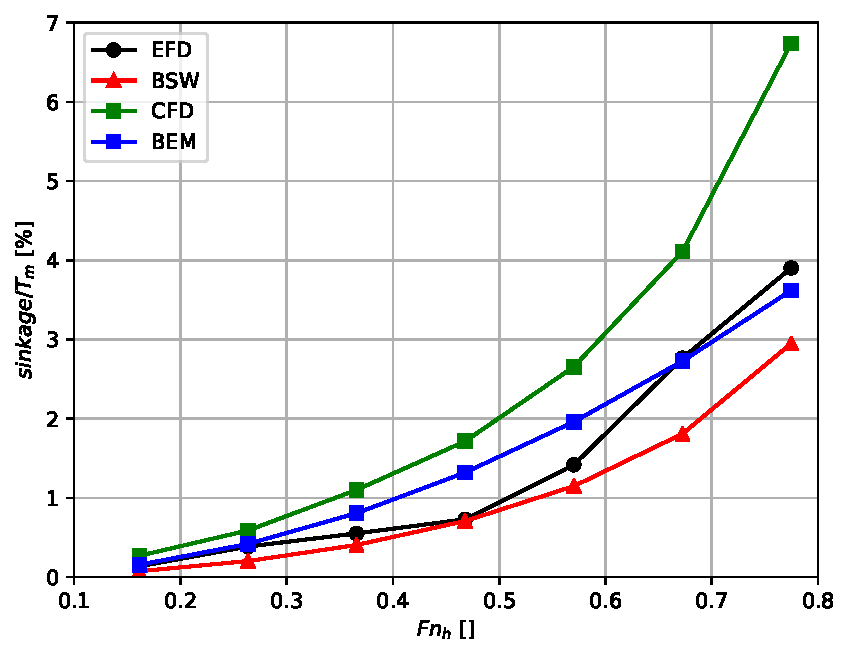
\includegraphics[width=0.9\linewidth]{figures/Example03_Beguin_MASHCON2013_WigleyHull}
	\caption{}
	\label{fig:example03beguinmashcon2013wigleyhull}
\end{figure}
\section{DTC in shallow water, MASHCON 2019 Case C1, C2 and C3}
\begin{figure}
	\centering
	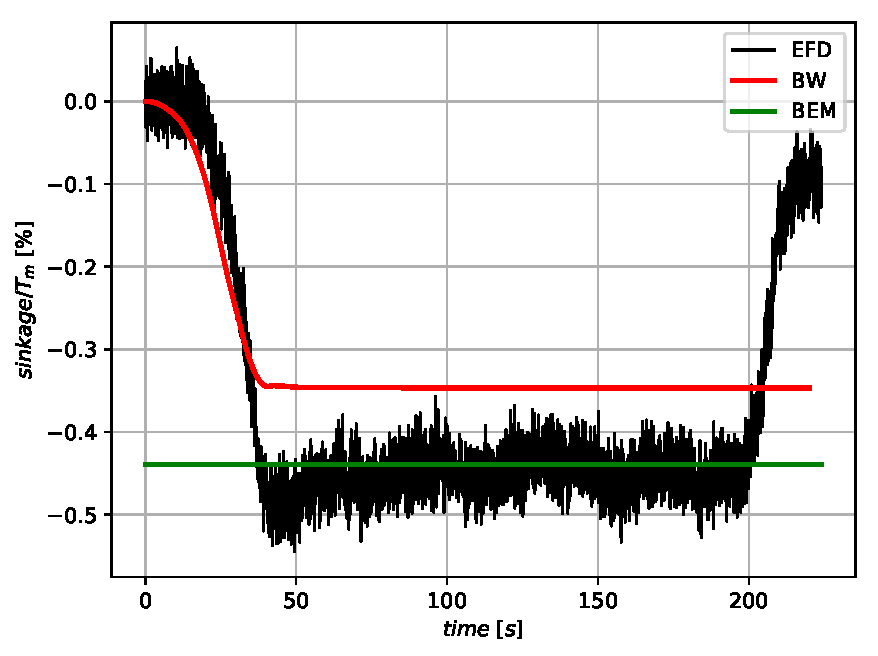
\includegraphics[width=0.9\linewidth]{figures/Example04_MASHCON2019_DTC_C1_Sinkage}
	\caption{}
	\label{fig:example04mashcon2019dtcc1sinkage}
\end{figure}
\begin{figure}
	\centering
	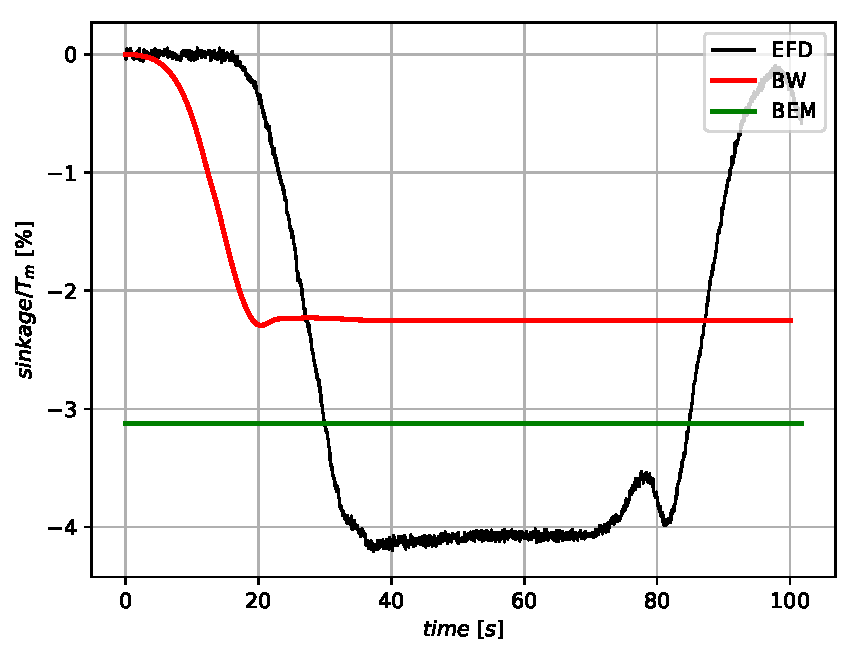
\includegraphics[width=0.9\linewidth]{figures/Example04_MASHCON2019_DTC_C2_Sinkage}
	\caption{}
	\label{fig:example04mashcon2019dtcc1sinkage}
\end{figure}
\begin{figure}
	\centering
	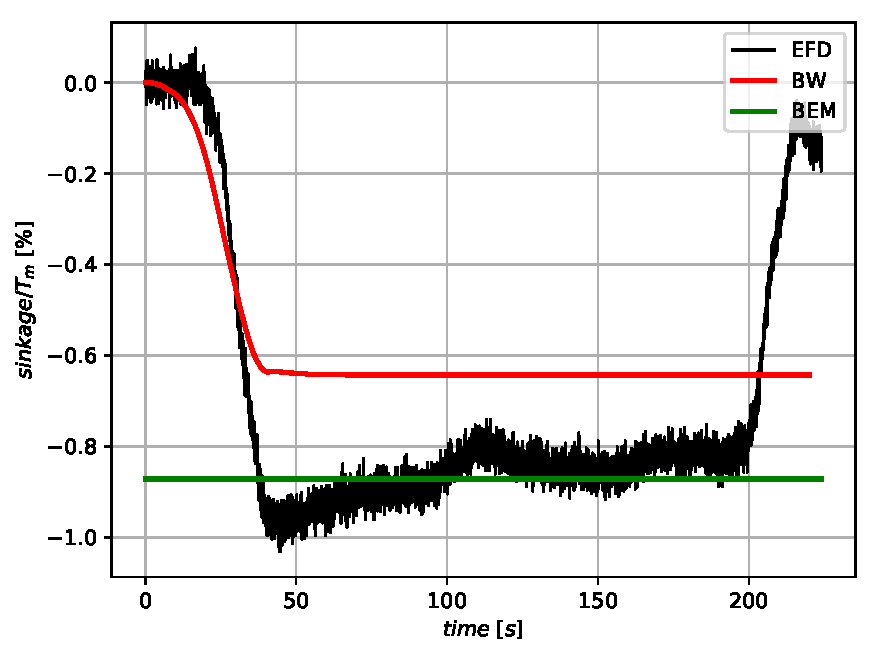
\includegraphics[width=0.9\linewidth]{figures/Example04_MASHCON2019_DTC_C3_Sinkage}
	\caption{$Fr_L = $, $Fr_h = $}
	\label{fig:example04mashcon2019dtcc1sinkage}
\end{figure}


\section{KCS in deep water, SIMMAN 2020 Case 3.1}
\section{KCS in shallow water, SIMMAN 2020 Case 4.1}

\end{document}
